\section{Příklad 1}
% Jako parametr zadejte skupinu (A-H)
\prvniZadani{C}

Metoda zjednodušování spočívá v nahrazování odporových sítí uvnitř obvodu \textit{ekvivalentními odpory}, které se z hlediska zbytku obvodu chovají stejně -- mají stejný odpor. Postupným zjednodušováním se tak dostaneme do stavu, kdy jsou všechny odpory v obvodu reprezentovány jedním ekvivalentním odporem $R_{ekv}$. Pomocí něj vypočítáme celkový proud v obvodu, na základě kterého pak zpětně dopočítáváme napětí a proudy na jednotlivých prvcích.

V zadaném obvodu můžeme ihned zjednodušit rezistory $R_{7}$ a $R_{8}$ na ekvivalentní odpor $R_{78}$, jehož hodnotu vypočítáme pomocí vztahu o odporu v paralelním zapojení:
\begin{equation} \label{eq:parallel}
    R_{78} = \frac{R_{7} R_{8}}{R_{7}+R_{8}}
\end{equation}
Podobně můžeme ihned zjednodušit také rezistory $R_{4}$ a $R_{5}$, které jsou zapojené v sérii, proto:
\[
    R_{45} = R_{4} + R_{5}
\]
Zdroje napětí $U_1$ a $U_2$ jsou zapojeny v sérii přímo za sebou, proto je můžeme zjednodušit na jeden zdroj o napětí
\[
    U_{12} = U_1 + U_2
\]
Výsledný obvod můžeme znázornit:
\begin{figure}[H]
    \centering
    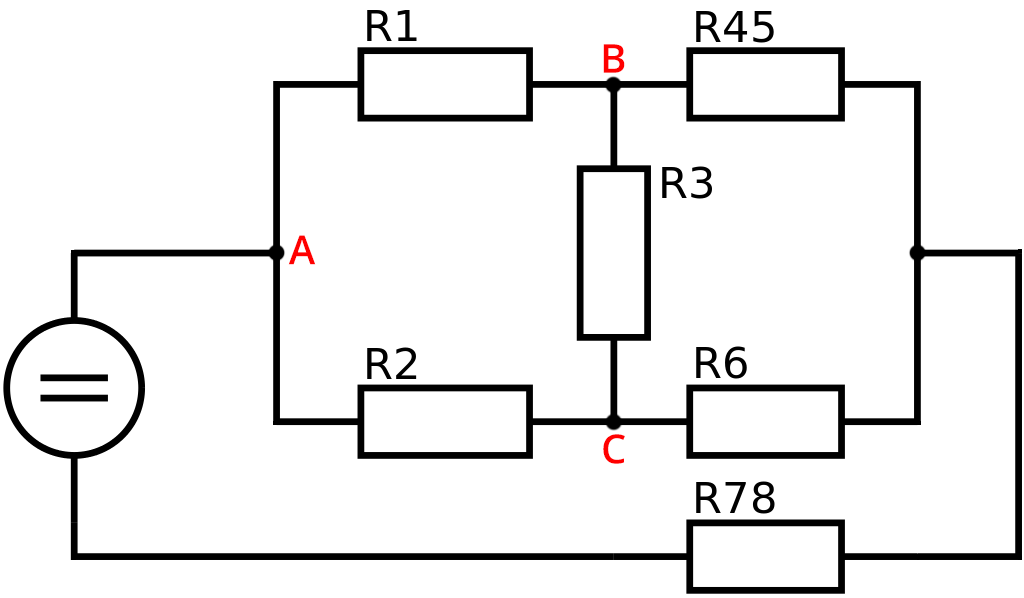
\includegraphics[width=7cm]{diagrams/Diagram1.png}
    \caption{Obvod se zjednodušenými $R_4,R_5,R_7,R_8,U_1,U_2$.}
    \label{fig:circ-1-1}
\end{figure}

Ve vzniklém obvodu tvoří soustava rezistorů $R_1$, $R_2$ a $R_3$ trojúhelník, který pro zjednodušení výpočtů převedeme na hvězdu (obdobně by se dalo počítat také s rezistory $R_3$, $R_{45}$ a $R_6$). Hvězdu budou tvořit tři rezistory $R_A$, $R_B$, $R_C$, jejichž hodnoty budou nastaveny tak, aby odpor mezi uzly \textcolor{red}{A}, \textcolor{red}{B} a \textcolor{red}{C}, ve kterých je hvězda připojena do obvodu, odpovídal odporu mezi těmito uzly v původním obvodu. Obvod s hvězdou znázorňuje obr. \ref{fig:circ-1-2}. Pro vzniklé rezistory platí vztahy:
\begin{equation} \label{eq:star}
R_A = \frac{R_1 R_2}{R_1+R_2+R_3},\,
R_B = \frac{R_1 R_3}{R_1+R_2+R_3},\,
R_C = \frac{R_2 R_3}{R_1+R_2+R_3}
\end{equation}
\begin{figure}[ht]
    \centering
    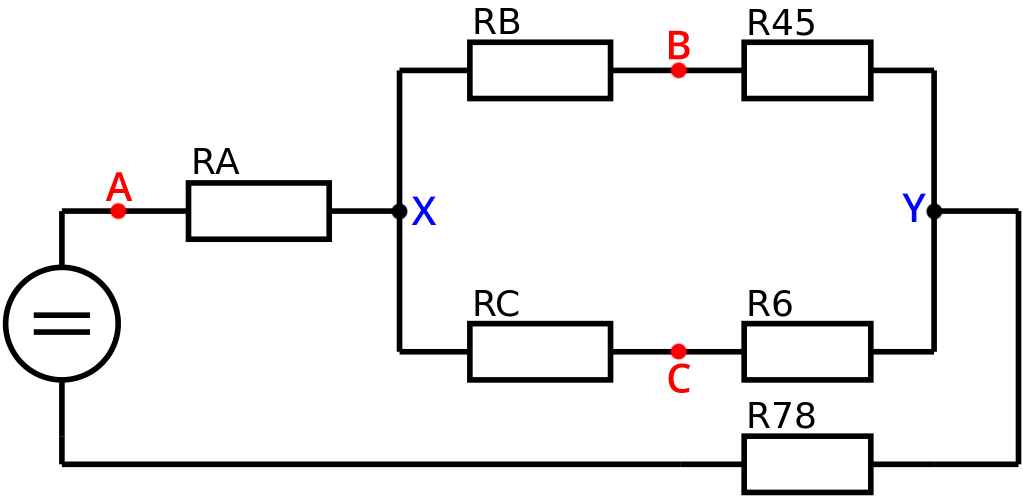
\includegraphics[width=7cm]{diagrams/Diagram2.png}
    \caption{Obvod s trojúhelníkem rezistorů převedeným na hvězdu. Odpor mezi uzly A, B, C vyznačenými červenou barvou odpovídá odporu mezi těmito uzly ve schématu na obrázku \ref{fig:circ-1-1}.}
    \label{fig:circ-1-2}
\end{figure}

Obdobnými kroky zjednodušíme část obvodu mezi uzly \textcolor{blue}{X} a \textcolor{blue}{Y}. Rezistory zapojené v sérii $R_B$ a $R_{45}$ můžeme nahradit rezistorem $R_{B45}$ s odporem $R_{B45} = R_B + R_{45}$, podobně pak zjednodušíme $R_C$ a $R_6$, jak ukazuje levá část obrázku \ref{fig:circ-1-3}. Mezi uzly \textcolor{blue}{X} a \textcolor{blue}{Y} jsou nyní dva rezistory zapojené paralelně, které můžeme zjednodušit na odpor $R_W$ pomocí vztahu ekvivalentního s \eqref{eq:parallel}:
\begin{equation}
    \label{eq:rw}
    \begin{gathered}
        \frac{1}{R_W} = \frac{1}{R_{B45}} + \frac{1}{R_{C6}} = \frac{1}{R_B+R_{45}} + \frac{1}{R_C+R_6} \\
        R_W = \frac{(R_B+R_{45})(R_C+R_6)}{R_B+R_{45}+R_C+R_6} = \frac{(R_B+R_4+R_5)(R_C+R_6)}{R_B+R_C+R_4+R_5+R_6}
    \end{gathered}
\end{equation} 

\begin{figure}[ht]
    \centering
    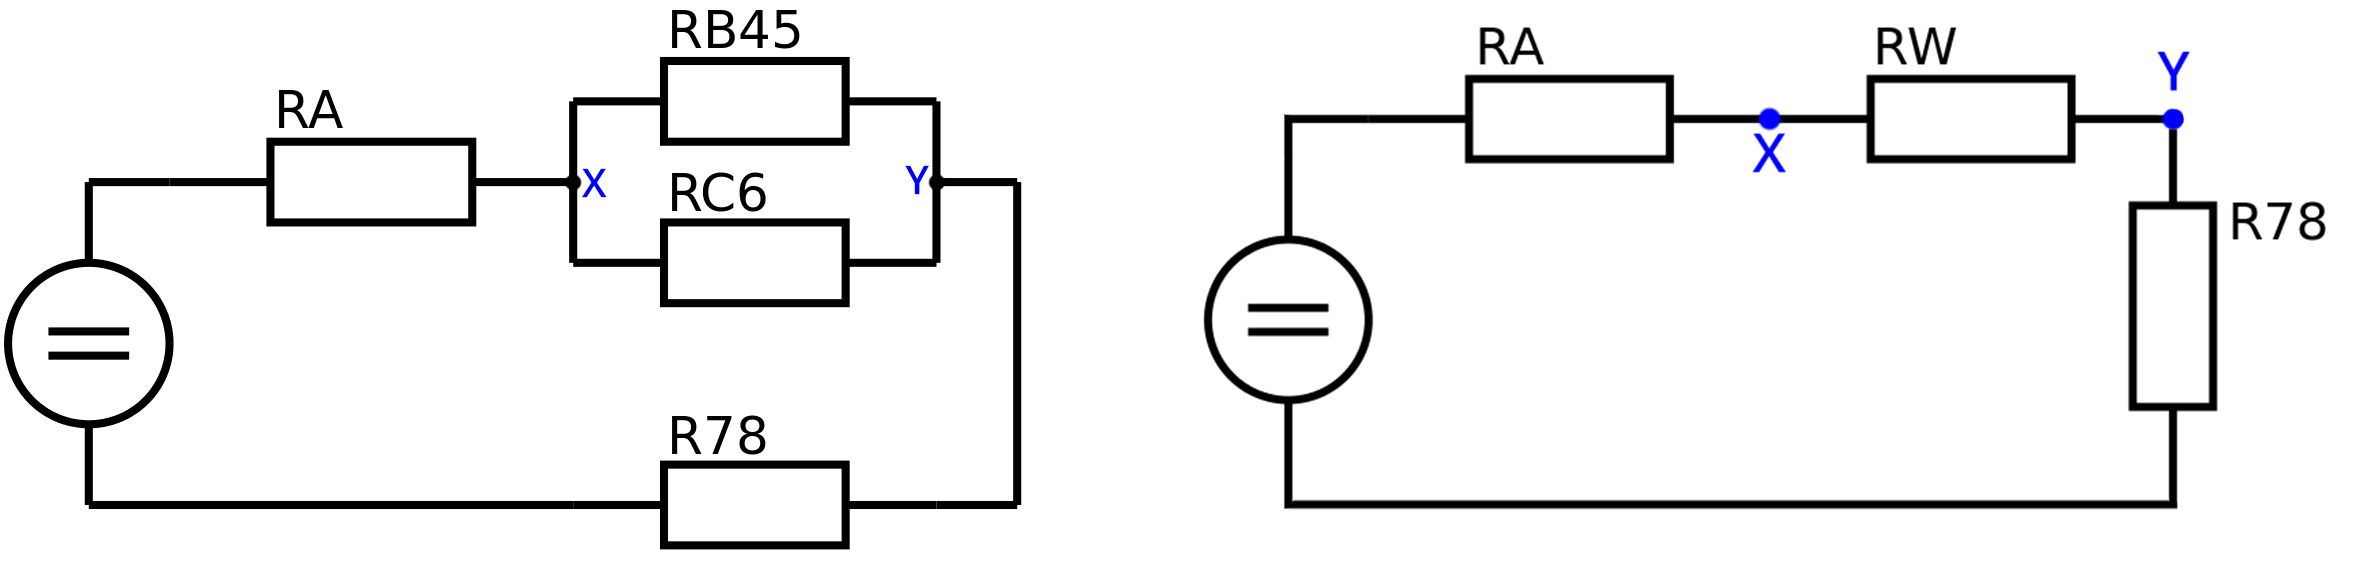
\includegraphics[width=14cm]{diagrams/Diagram3.png}
    \caption{Další kroky zjednodušování.}
    \label{fig:circ-1-3}
\end{figure}

Nyní v obvodu zůstaly pouze tři odpory v sérii, celkový ekvivalentní odpor $R_{ekv}$ je tak jejich součtem:
\[
    R_{ekv} = R_A + R_W + R_{78} = \frac{R_1 R_2}{R_1 + R_2 + R_3} + \frac{(R_B+R_4+R_5)(R_C+R_6)}{R_B+R_C+R_4+R_5+R_6} + \frac{R_{7} R_{8}}{R_{7}+R_{8}}
\]

Aby nebyl výsledný výraz příliš komplikovaný, pomocné odpory $R_B$, $R_C$ a $R_W$ si nyní podle vztahů \eqref{eq:star} a \eqref{eq:rw} spočítáme:
\begin{gather*}
    R_B = \frac{450\cdot 190}{450+810+190} = \frac{1710}{29}\ \Omega \approx \SI{58.9655}{\ohm}\\
    R_C = \frac{810\cdot 190}{450+810+190} = \frac{3078}{29}\ \Omega \approx \SI{106.1379}{\ohm}\\
    R_W = \frac{(\frac{1710}{29} + 220 + 220)(\frac{3078}{29} + 720)}{\frac{1710}{29} + \frac{3078}{29} + 220 + 220 + 720} = \frac{\num{86668065}}{\num{278603}}\ \Omega \approx \SI{311.08087}{\ohm}
\end{gather*}
Dosadíme do zjištěného vztahu:
\begin{gather*}
    R_{ekv} = \frac{450\cdot 810}{450+810+190} + \frac{\num{86668065}}{\num{278603}} + \frac{260\cdot 180}{260+180} \\
    \\
    \mathbf{R_{ekv} \approx \SI{668.8238}{\ohm}}
\end{gather*}

S pomocí zjištěného ekvivalentního odporu celé odporové sítě $R_{ekv}$ a ekvivalentního napětí v obvodu $U_{12}$ můžeme použitím Ohmova zákona spočítat celkový proud v obvodu:
\[
    I = \frac{U_{12}}{R_{ekv}} = \frac{180}{\num{668.8238}} \approx \SI{0.26913}{A}
\]

Nyní opět pomocí Ohmova zákona a základních znalostí o chování proudu a napětí při větvení obvodu zpětně spočítáme napětí a proud na zjednodušených ekvivalentních odporech a poté uvnitř částí obvodu, které byly zjednodušeny. Hledanými hodnotami jsou napětí a proud na rezistoru $R_5$. $R_5$ je v počátku součástí náhradního odporu $R_W$. Napětí na tomto odporu (mezi uzly \textcolor{blue}{X} a \textcolor{blue}{Y}) je stejné jako napětí na $R_{B45}$, protože $R_W$ odpovídá dvěma paralelně zapojeným rezistorům, v tomto případě se napětí nedělí. Podle tohoto napětí spočítáme proud procházející náhradním odporem $R_{B45}$, a tedy i hledaný $R_5$, protože $R_{B45}$ odpovídá odporům zapojeným v sérii, kdy se proud nedělí. Podle proudu $I_{R_5}$ pak v závěru spočítáme napětí $U_{R_5}$.

\begin{gather*}
    U_{R_{B45}} = U_{R_W} = IR_W = \frac{U_{12}}{R_{ekv}} \cdot R_W \\
    I_{R_5} = I_{R_{B45}} = \frac{U_{R_{B45}}}{R_{B45}} = \frac{U_{R_{B45}}}{R_B + R_{45}} = \frac{U_{12} R_W}{R_{ekv}(R_B+R_4+R_5)} = \frac{180\cdot \num{311.08087}}{\num{668.8238}\cdot (\num{58.9655}+220+220)} \\
    \mathbf{I_{R_5} \approx \SI{0.167789}{\ampere}} \\
    \\
    U_{R_5} = I_{R_5} R_5 \approx \num{0.167789}\cdot 220 \\
    \mathbf{U_{R_5} \approx \SI{36.91358}{\volt}}
\end{gather*}